% 由 final_document/PHYSICAL_GAME_RULES.md 同步；編譯：cd final_document && xelatex PHYSICAL_GAME_RULES.tex
\documentclass[11pt]{article}
\usepackage[a4paper,margin=2cm]{geometry}
\usepackage{fontspec}
\usepackage{xeCJK}
\usepackage{booktabs}
\usepackage{enumitem}
\usepackage{graphicx}

\graphicspath{{../}}

\setmainfont{Times New Roman}
\IfFontExistsTF{Songti TC}{
  \setCJKmainfont{Songti TC}
  \setCJKsansfont{Heiti TC}
}{
  \setCJKmainfont{FandolSong}
  \setCJKsansfont{FandolHei}
}

\setlist{nosep,leftmargin=1.8em}
\setlist[enumerate,1]{label=\arabic*., leftmargin=2em}
\setlist[enumerate,2]{label=\arabic{enumi}.\arabic*., leftmargin=2.2em}

\newcommand{\term}[1]{\textbf{#1}}
\newcommand{\coord}[1]{\texttt{#1}}

\begin{document}

{\LARGE\bfseries 防守題評分方式\par}
\vspace{0.8em}

\section*{零、重點內容}

本題的重點為第一大點至第四大點，第五大點後僅是防守球員移動方法，不需細看。

\section*{一、遊戲目的}

進攻方必須在指定回合數內，利用盤帶、無球跑位及傳球改變站位，最後完成射門得分。

\begin{itemize}
  \item 射門進球：立即過關。
  \item 盤帶踏入防守格、移動階段結束時貼身壓迫條件成立、傳球失敗、射門未進：立即失敗。
  \item 回合用盡仍未進球：失敗。
\end{itemize}

\section*{二、場地與座標}

\subsection*{2.1 棋盤}

\begin{itemize}
  \item 場地為 \term{7 格寬 $\times$ 8 格深}（實體格線或等價標記）。
  \item 橫向座標為 \coord{x = 0～6}，由左至右增加。
  \item 縱向座標為 \coord{y = 0～7}，越接近 \coord{y=7} 越接近對方球門。
  \item 任一球員的位置以 \coord{(x,y)} 表示。
\end{itemize}

\subsection*{2.2 球門}

球門位於最深一排 \coord{y=7}，包含三格：

\begin{itemize}
  \item 左柱：\coord{(2,7)}
  \item 中路：\coord{(3,7)}
  \item 右柱：\coord{(4,7)}
\end{itemize}

射門目標必須對應上述球門區。守門員站位亦限於這三格。

\subsection*{2.3 移動距離}

「移動 1 格」採八方向計算，包括上、下、左、右及四個斜向。

\section*{三、球員與佔位}

違反以下規則者黃牌一張。

\subsection*{3.1 持球者}

\begin{itemize}
  \item 任何時刻僅一名進攻球員持球。
  \item 開局站位、持球者由關卡指定。
  \item 傳球成功後，接球者立即成為新持球者。
\end{itemize}

\subsection*{3.2 格子佔用}

格子上不得有兩名或以上球員。

\subsection*{3.3 所屬方格}

\begin{itemize}
  \item 每名球員在任何時刻屬於一個指定方格。
  \item 雙腳必須站在該格內。
  \item 在非移動階段時，球員不得擅自離開原所屬格。
\end{itemize}

\section*{四、回合結構}

\subsection*{4.1 回合計數}

正式關卡均以 \term{8 回合}為上限（關卡另有明文者從其規定）。關卡的步驟包含以下階段，上一階段結束時進入下一階段，且在每個階段開始時關主皆會宣告並請小隊員選擇執行或跳過。選擇執行時關主會確認成功與否。

\subsection*{4.2 射門階段}

\begin{itemize}
  \item 只要選擇射門，回合立即結束。
  \item 整顆球進入球門範圍內則得分。
  \item 持球者必須位於 \coord{y $\geq$ 4} 才能射門。
\end{itemize}

\subsection*{4.3 移動階段}

在此階段所有隊員皆可移動，每位小隊員僅能移動一次。持球者移動定義為盤帶，非持球者移動定義為無球跑位。兩者合法操作分別如下：

\begin{itemize}
  \item 目標在棋盤內；
  \item 與原位置相距恰好 1 格；
  \item 關卡未禁止盤帶。
\end{itemize}

惟盤帶時需做關主指定繞錐帶球動作，過程中不得碰到任何角錐（待定）。

\subsection*{4.4 傳球階段}

傳球階段由以下傳球相關規定認定。

\subsubsection*{4.4.1 傳球程序}

持球者宣告接球隊友。

\subsubsection*{4.4.2 傳球結束}

同時符合：

\begin{enumerate}
  \item 接球者需觸球；
  \item 球停止移動；
\end{enumerate}

結束後：

\begin{enumerate}
  \item 接球者成為持球者；
  \item 回合結束。
\end{enumerate}

\subsection*{4.5 結束回合}

\begin{itemize}
  \item 防守方統一移動；
  \item 回合數 $+1$。
\end{itemize}

\section*{五、防守球員共同規則}

\subsection*{5.1 防守反應與重疊結算}

防守反應時，依下列程序結算：

\begin{enumerate}
  \item \textbf{計算首選}：每位防守者依角色規則算出首選目標格，以及本次反應的最大步數。
  \item \textbf{全體離格}：所有防守者同時離開原格。
  \item \textbf{依優先序佔格}：門將 $\rightarrow$ 大閘 $\rightarrow$ 逼搶員 $\rightarrow$ 攔截者 $\rightarrow$ 影子。同角色依防守者編號（id）字典序，較前者先佔。
  \item \textbf{後佔者可用先佔者騰出的格}：因已全體離格，先結算者未選的原格，後結算者可以進入。
  \item \textbf{不得站入進攻球員所在格}。
  \item \textbf{不允許兩名防守者重疊}。
\end{enumerate}

\subsubsection*{本次最大步數}

\vspace{0.3em}
\begin{tabular}{@{}lll@{}}
\toprule
\textbf{角色} & \textbf{最大步數} & \textbf{角色區域} \\
\midrule
門將 & 1 & 僅球門三格 \coord{(2,7)(3,7)(4,7)} \\
大閘 & 1 & 僅其固定橫線 \coord{y} \\
逼搶員 & 2 & 全場（不可進球門格、不可佔持球者格） \\
攔截者 & 距卡位目標 $\geq 2$ 則 2，否則 1 & 全場（不可進球門格） \\
影子 & 1 & 全場（不可進球門格；不可站到被盯者球側） \\
定點大閘 & 0 & 關卡指定格，永不離格 \\
\bottomrule
\end{tabular}

\vspace{0.4em}
\noindent
距離採八方向（切比雪夫距離）：斜走 1 格也算 1 步。

\subsubsection*{落點判定}

每位防守者依序決定落點：

\begin{enumerate}
  \item 若首選格空 $\rightarrow$ 站首選；
  \item 否則，只在「距原位 $\leq$ 本次最大步數」且符合角色區域的\textbf{空格}中選替代格；
  \item 替代格排序（愈前愈優先，全部為硬性比較，無裁量）：
  \begin{enumerate}
    \item 落在該角色偏好路線上（攔截者：傳球線中段格；影子：被盯者$\rightarrow$球門中心路線上的格；其餘角色無此項）；
    \item 距首選目標較近；
    \item 不往比首選更淺的 \coord{y} 後退；
    \item 距原位較近（移動較短）；
    \item \coord{y} 較大，再比 \coord{x} 較小；
  \end{enumerate}
  \item 若合法範圍內沒有空格 $\rightarrow$ 若原位仍空則留在原位；定點者永遠留在原位。
\end{enumerate}

\textbf{禁止}為了避開重疊而：

\begin{itemize}
  \item 超過該角色本次最大步數；
  \item 離開大閘的固定橫線；
  \item 讓非門將進入球門三格；
  \item 讓門將離開球門三格；
  \item 佔用定點大閘的格子。
\end{itemize}

\section*{六、防守角色}

\subsection*{6.1 瘋狗逼搶員（Presser）}

\begin{itemize}
  \item 每次防守反應最多移動 2 格；
  \item 可直走或斜走；
  \item 朝持球者靠近；
  \item 不會主動站入持球者所在格，而會停在鄰近位置施壓；
  \item 不會越過持球者所在的縱深線（不得使自己的 \coord{y} 大於持球者的 \coord{y}）。
\end{itemize}

\textbf{貼身壓迫：}

\begin{itemize}
  \item 若行動開始時逼搶員已與持球者相鄰，持球者選擇結束回合或在貼身狀態下硬盤，且行動後仍未擺脫相鄰範圍，\term{立即判定被搶斷，關卡失敗}；
  \item 及時傳球可解除原持球者所受的貼身判定。
\end{itemize}

逼搶員在傳球／射門時，只能在自己的格內實際攔截或封堵，不自動截斷。

\begin{center}
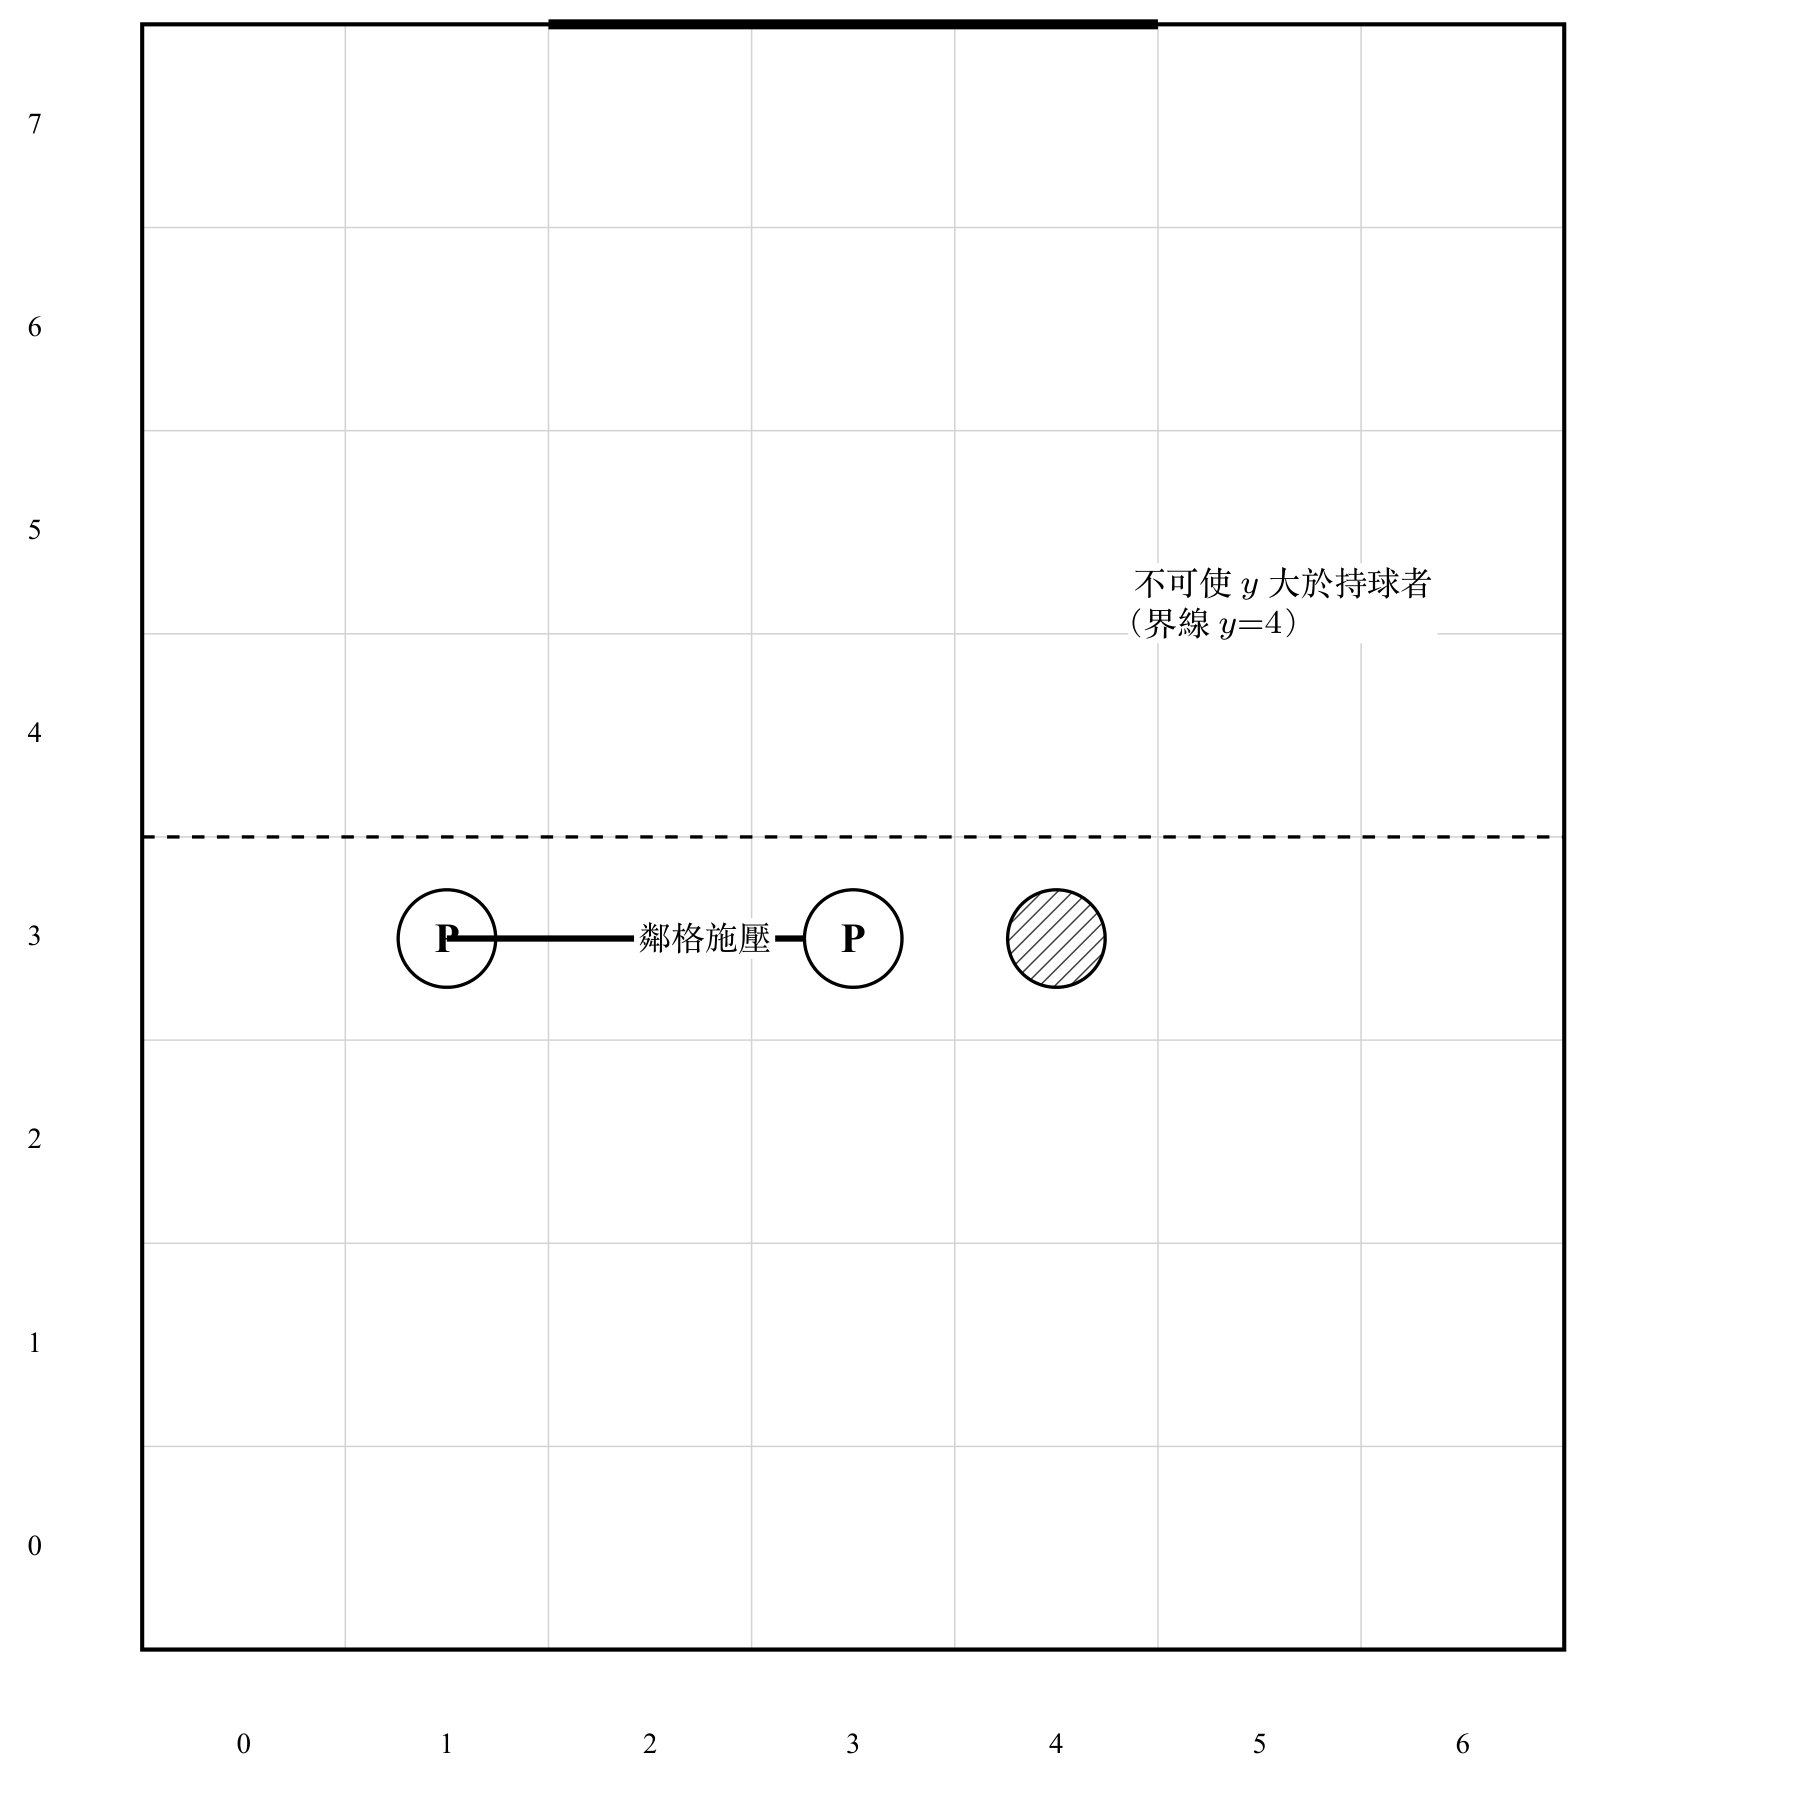
\includegraphics[width=0.82\textwidth]{defender_figures/presser.png}
\end{center}

\subsection*{6.2 區域大閘（Block）}

\begin{itemize}
  \item 每名大閘有一條固定橫線 \coord{y}；
  \item 不向前或向後移動；
  \item 每次反應最多橫移 1 格；
  \item 目標是站到「球的位置—球門中心 \coord{(3,7)}」連線穿過其橫線的位置；
  \item 若首選格被佔，依第五章重疊結算，在同一橫線、且距原位 $\leq 1$ 格的空格中改站。
\end{itemize}

\textbf{定點大閘（anchored）：}

\begin{itemize}
  \item 完全不移動，全程留在關卡指定格；
  \item 傳球／射門時仍可在該格內實際攔截或封堵。
\end{itemize}

\begin{center}
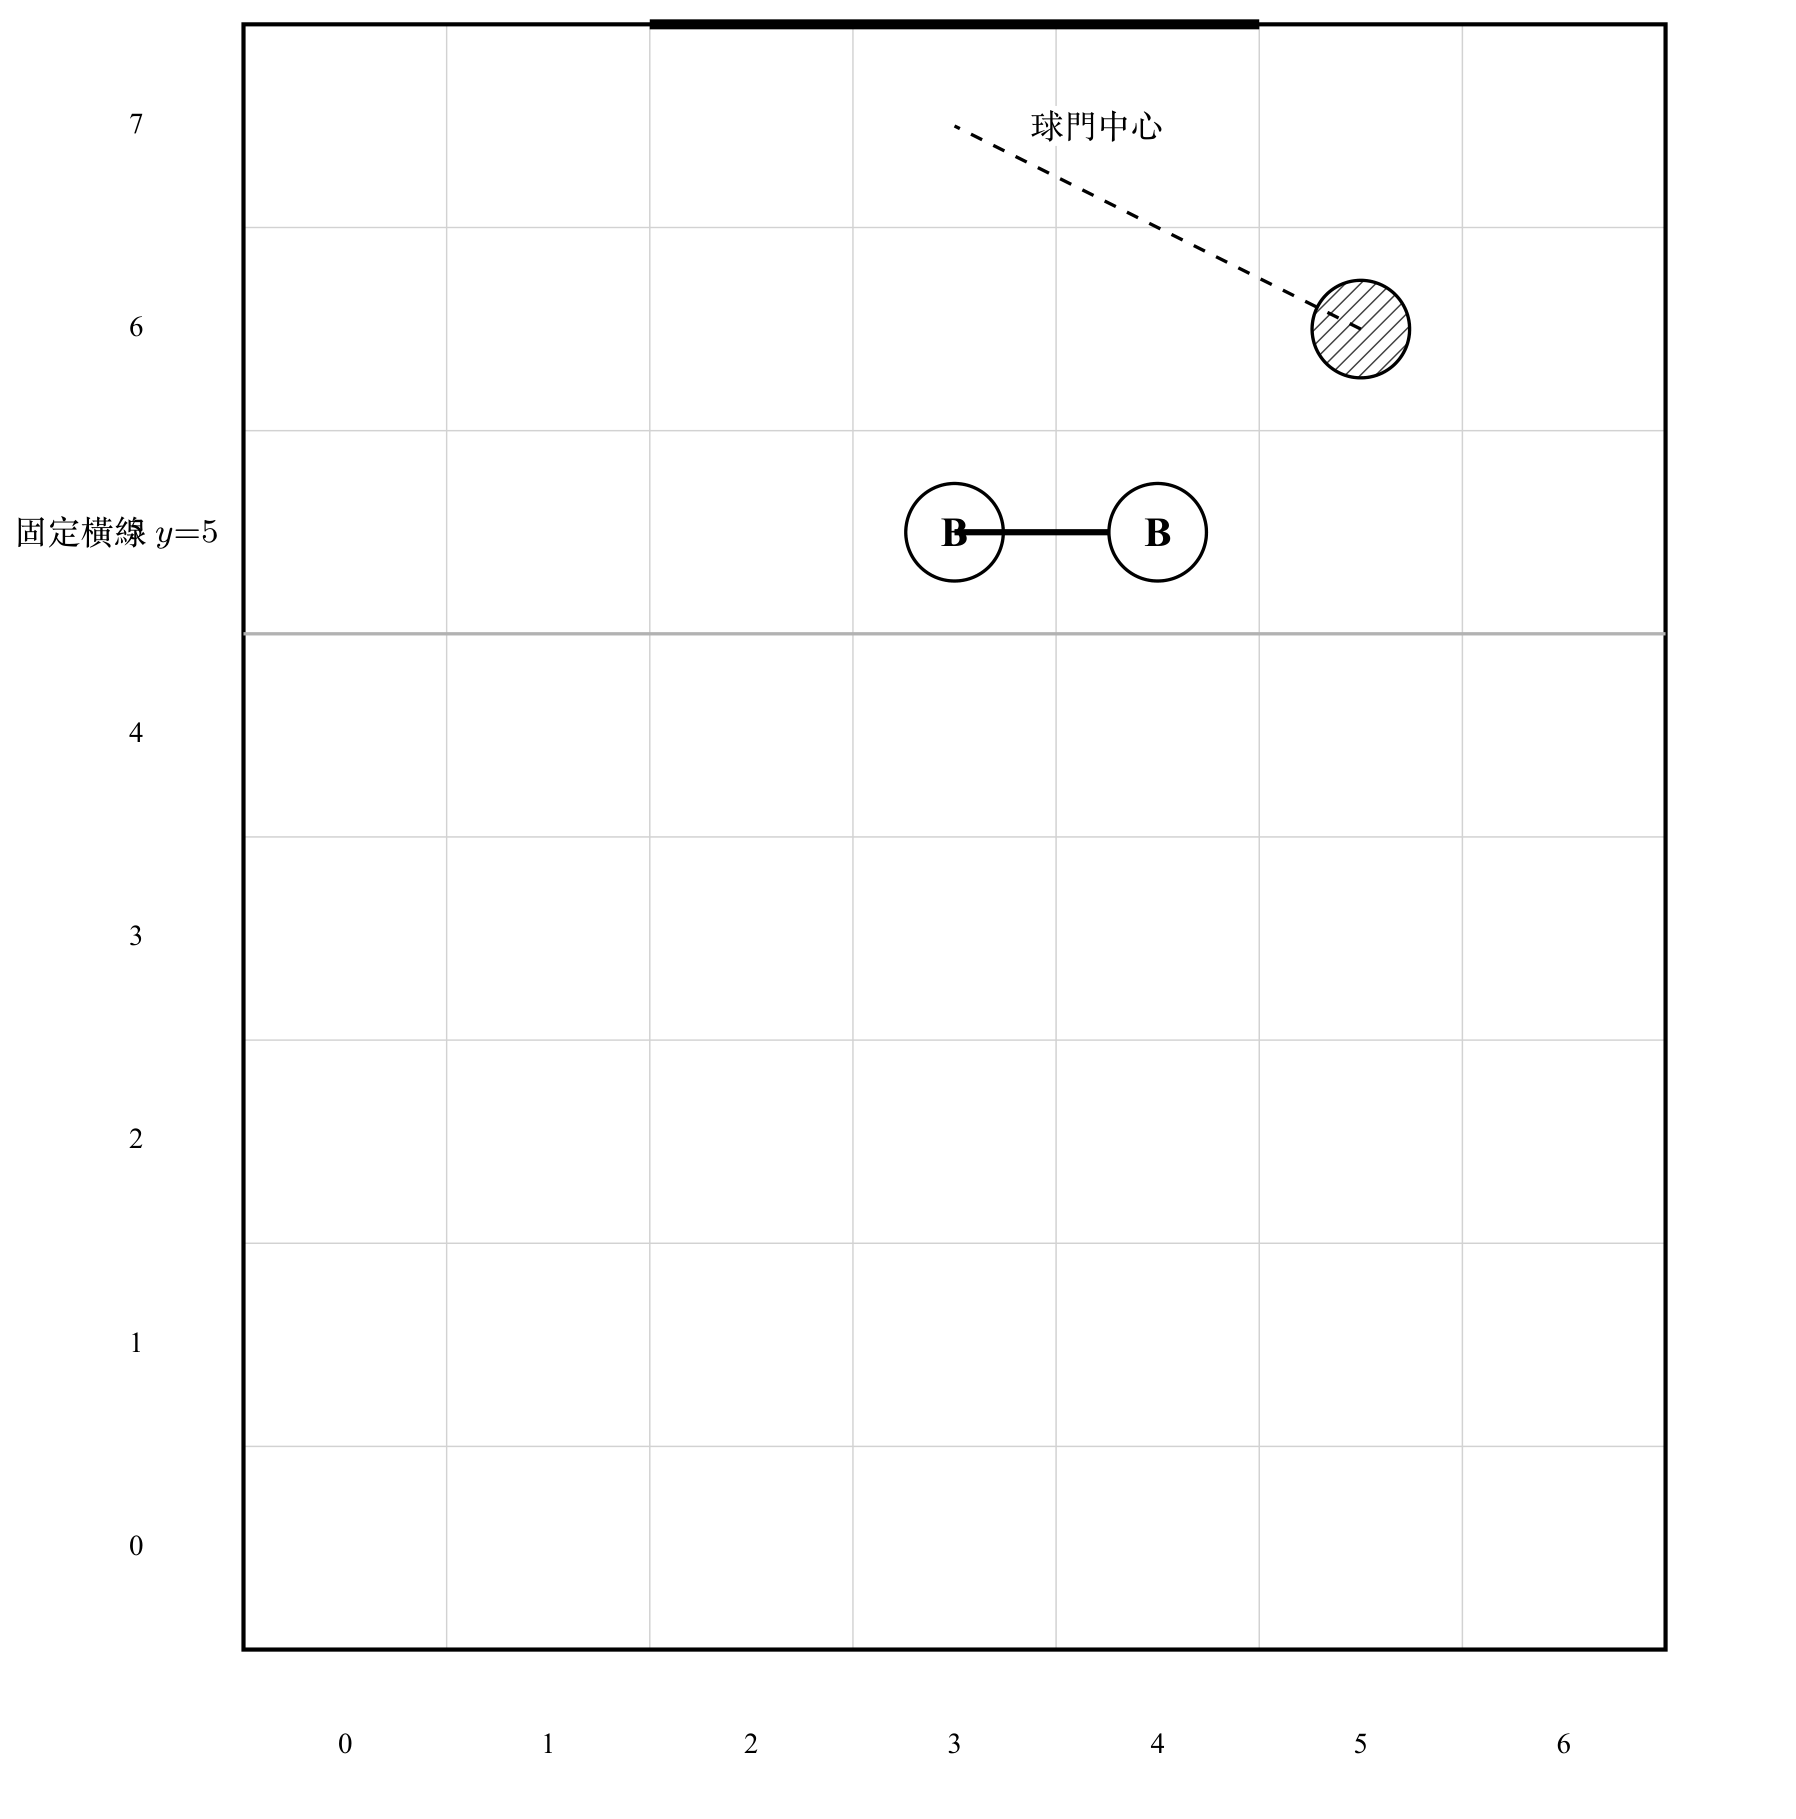
\includegraphics[width=0.82\textwidth]{defender_figures/block.png}
\end{center}

\subsection*{6.3 影子盯人者（Shadow）}

\begin{itemize}
  \item 每名影子固定盯一名進攻球員；
  \item 未預先指定時，開局選擇最近的進攻球員；
  \item 盯人關係確立後不任意更換；
  \item 每次防守反應移動最多 1 格；
  \item 目標格為被盯球員朝球門中心方向的下一格；
  \item 不主動站到被盯球員本人所在格；
  \item 不站到被盯球員的球側，也就是不站在比被盯者更小的 \coord{y}；
  \item 最高只到 \coord{y=6}，不進入球門格。
\end{itemize}

影子在跑位或盤帶的軟階段不動，只會在傳球或結束回合後跟上。

\begin{center}
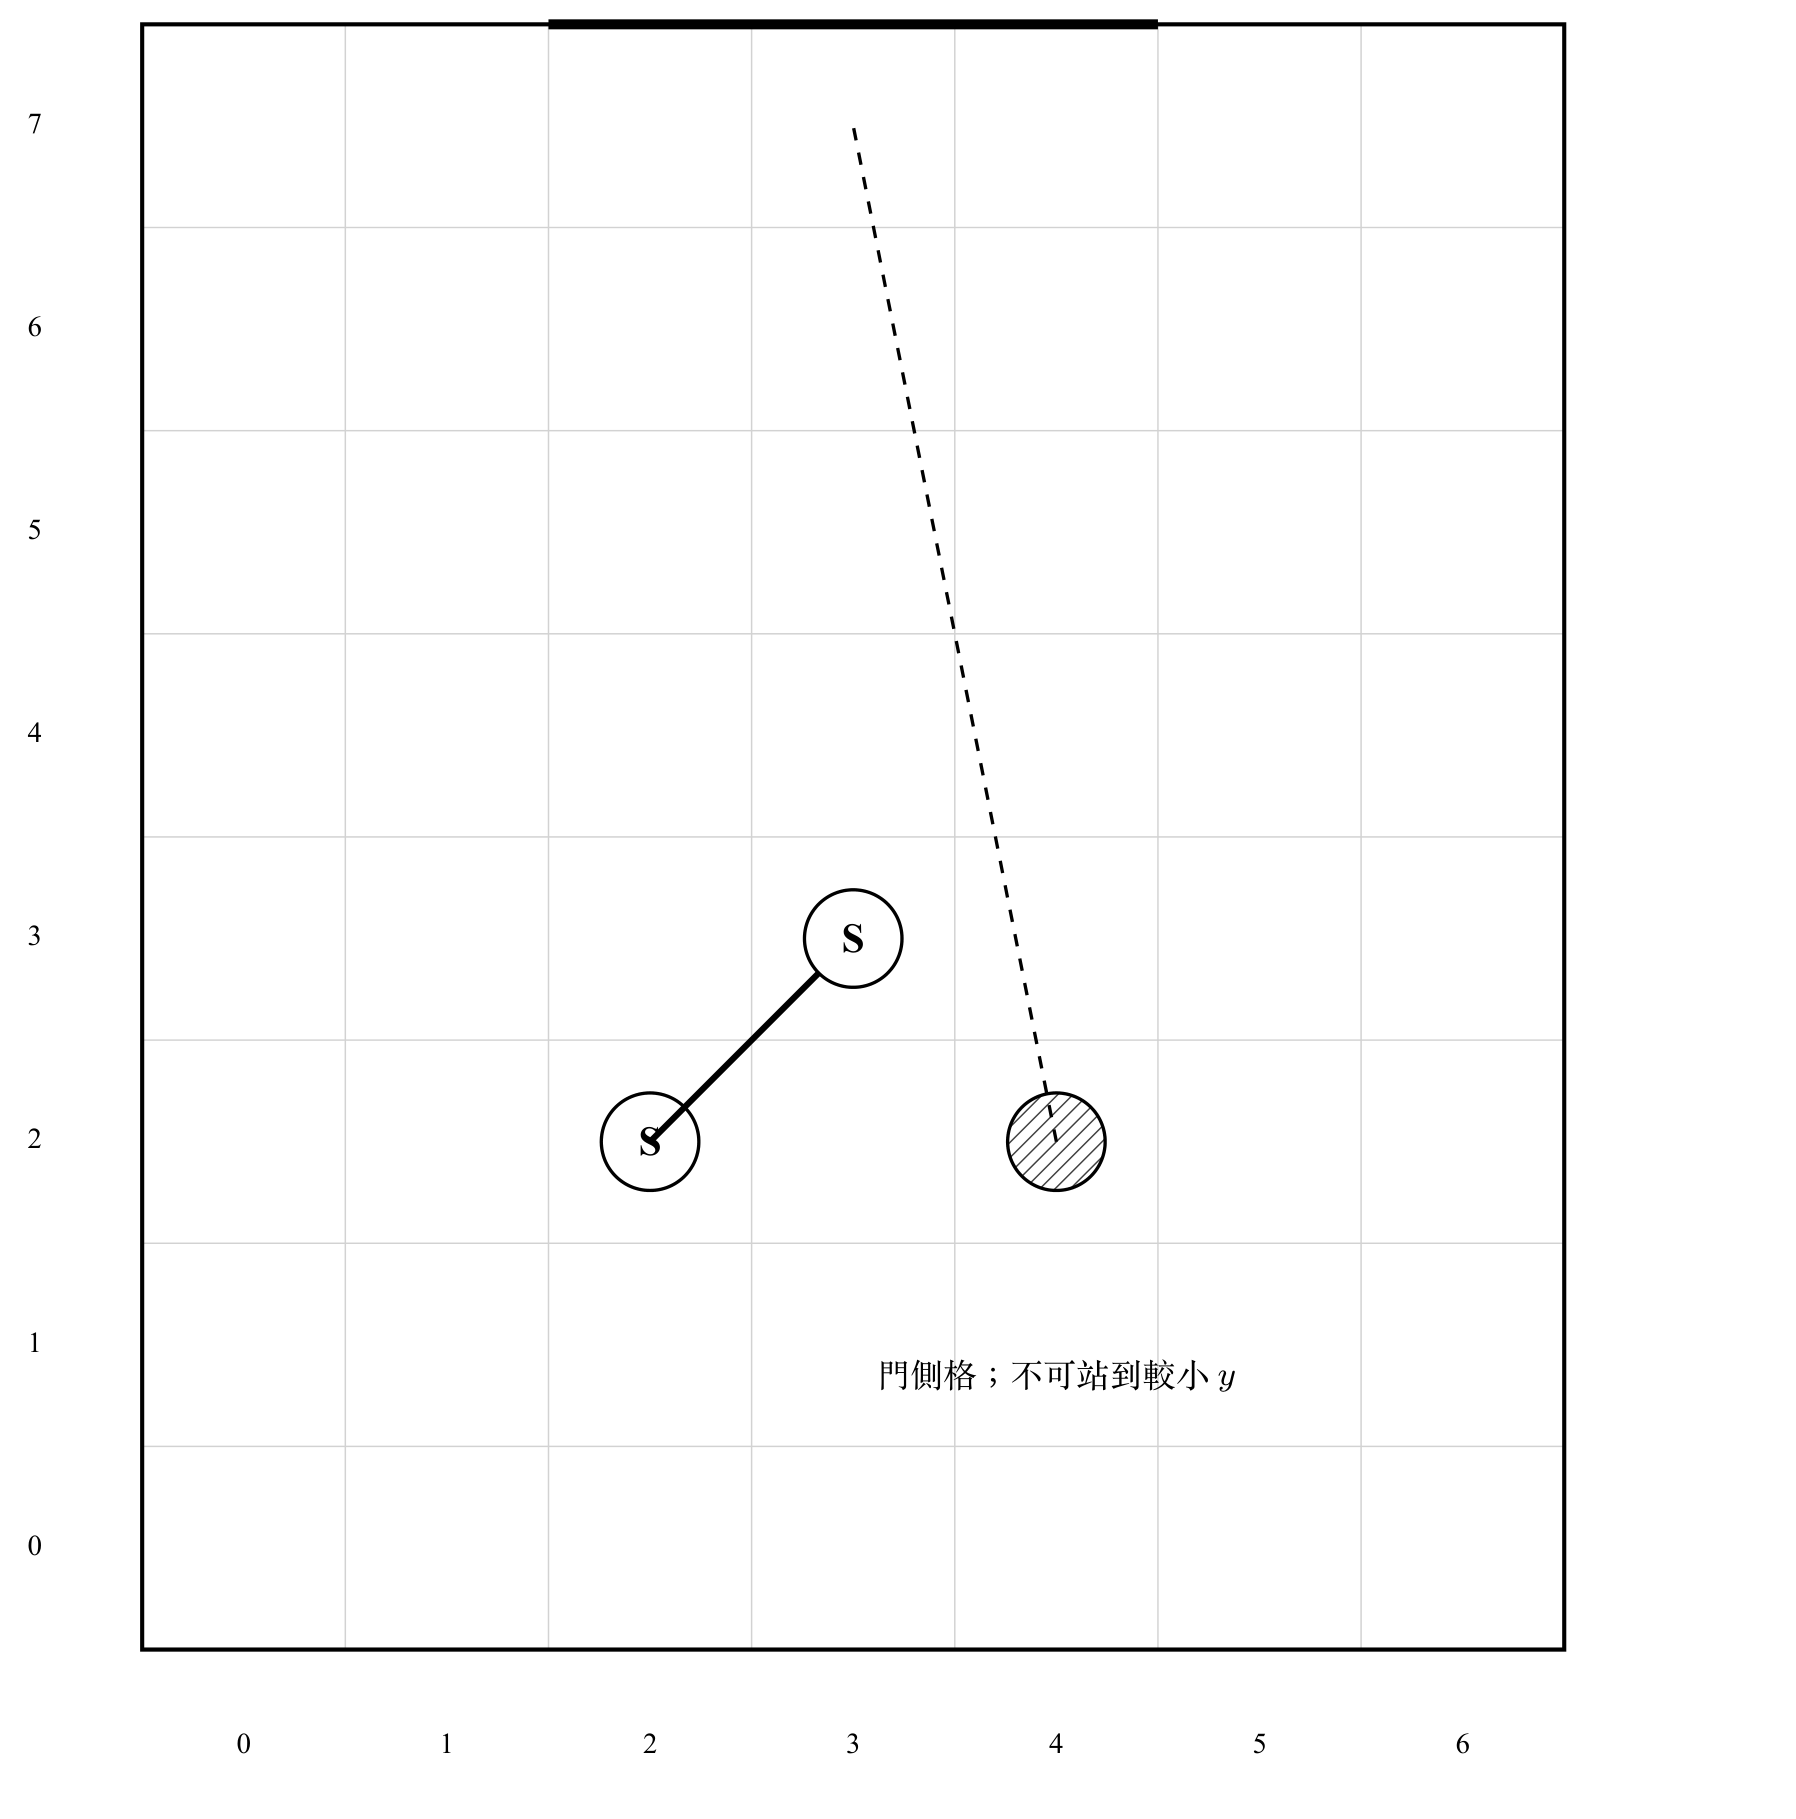
\includegraphics[width=0.82\textwidth]{defender_figures/shadow.png}
\end{center}

\subsection*{6.4 路線攔截者（Interceptor）}

\begin{itemize}
  \item 先排除目前持球者；
  \item 在其餘進攻球員中，優先選擇 \coord{y} 最大、最接近球門者；
  \item 若危險程度相同，優先選擇較接近持球者者；
  \item 以持球者至該球員的傳球線中段作為卡位目標；
  \item 距離目標較遠時最多移動 2 格，較近時移動 1 格；
  \item 若首選格被佔，依第五章重疊結算，優先改站同一傳球線上、且在本次步數內的其他空格。
\end{itemize}

攔截者站在預判路線上\textbf{不}自動令傳球失敗；必須在場上實際碰到或控制球。

\begin{center}
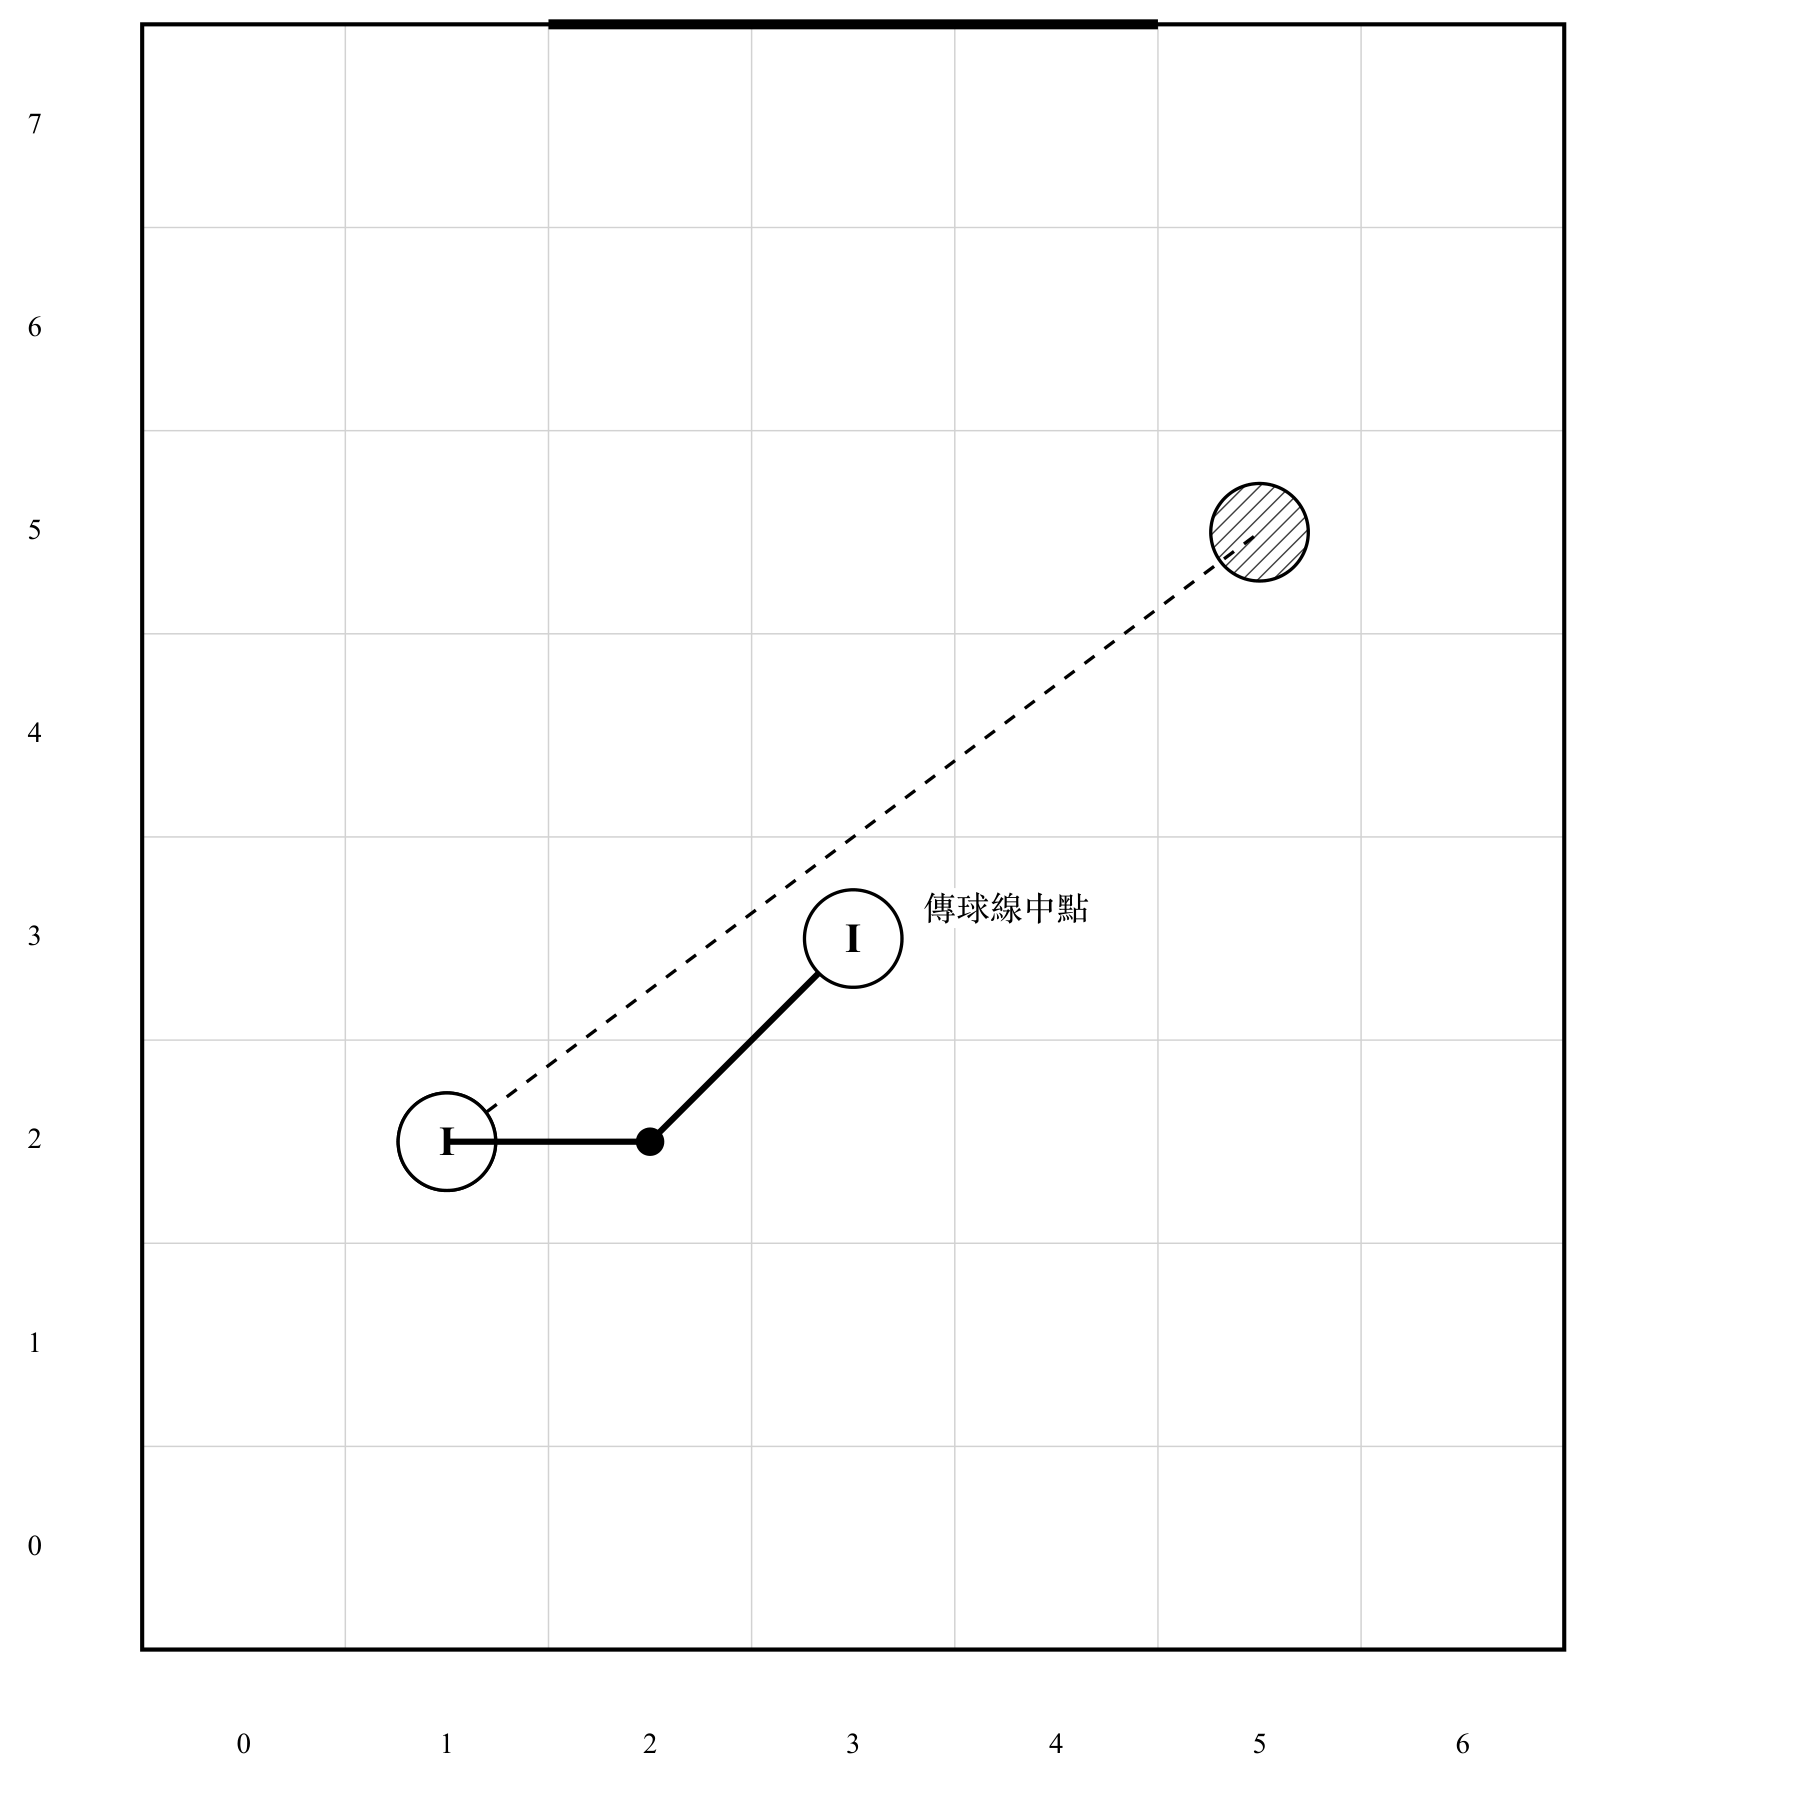
\includegraphics[width=0.82\textwidth]{defender_figures/interceptor.png}
\end{center}

\subsection*{6.5 守門員（Goalkeeper）}

\begin{itemize}
  \item 只能站在三個球門格 \coord{(2,7)}、\coord{(3,7)}、\coord{(4,7)}；
  \item 每次防守反應最多橫移 1 格；
  \item 球在左側時向 \coord{(2,7)} 靠近；
  \item 球在中路時向 \coord{(3,7)} 靠近；
  \item 球在右側時向 \coord{(4,7)} 靠近；
  \item 不論球距離球門多遠，都會跟隨球的橫向位置。
\end{itemize}

門將站在某一球門格\textbf{不}自動撲出；射門時必須實際完成撲救或漏球。

\begin{center}
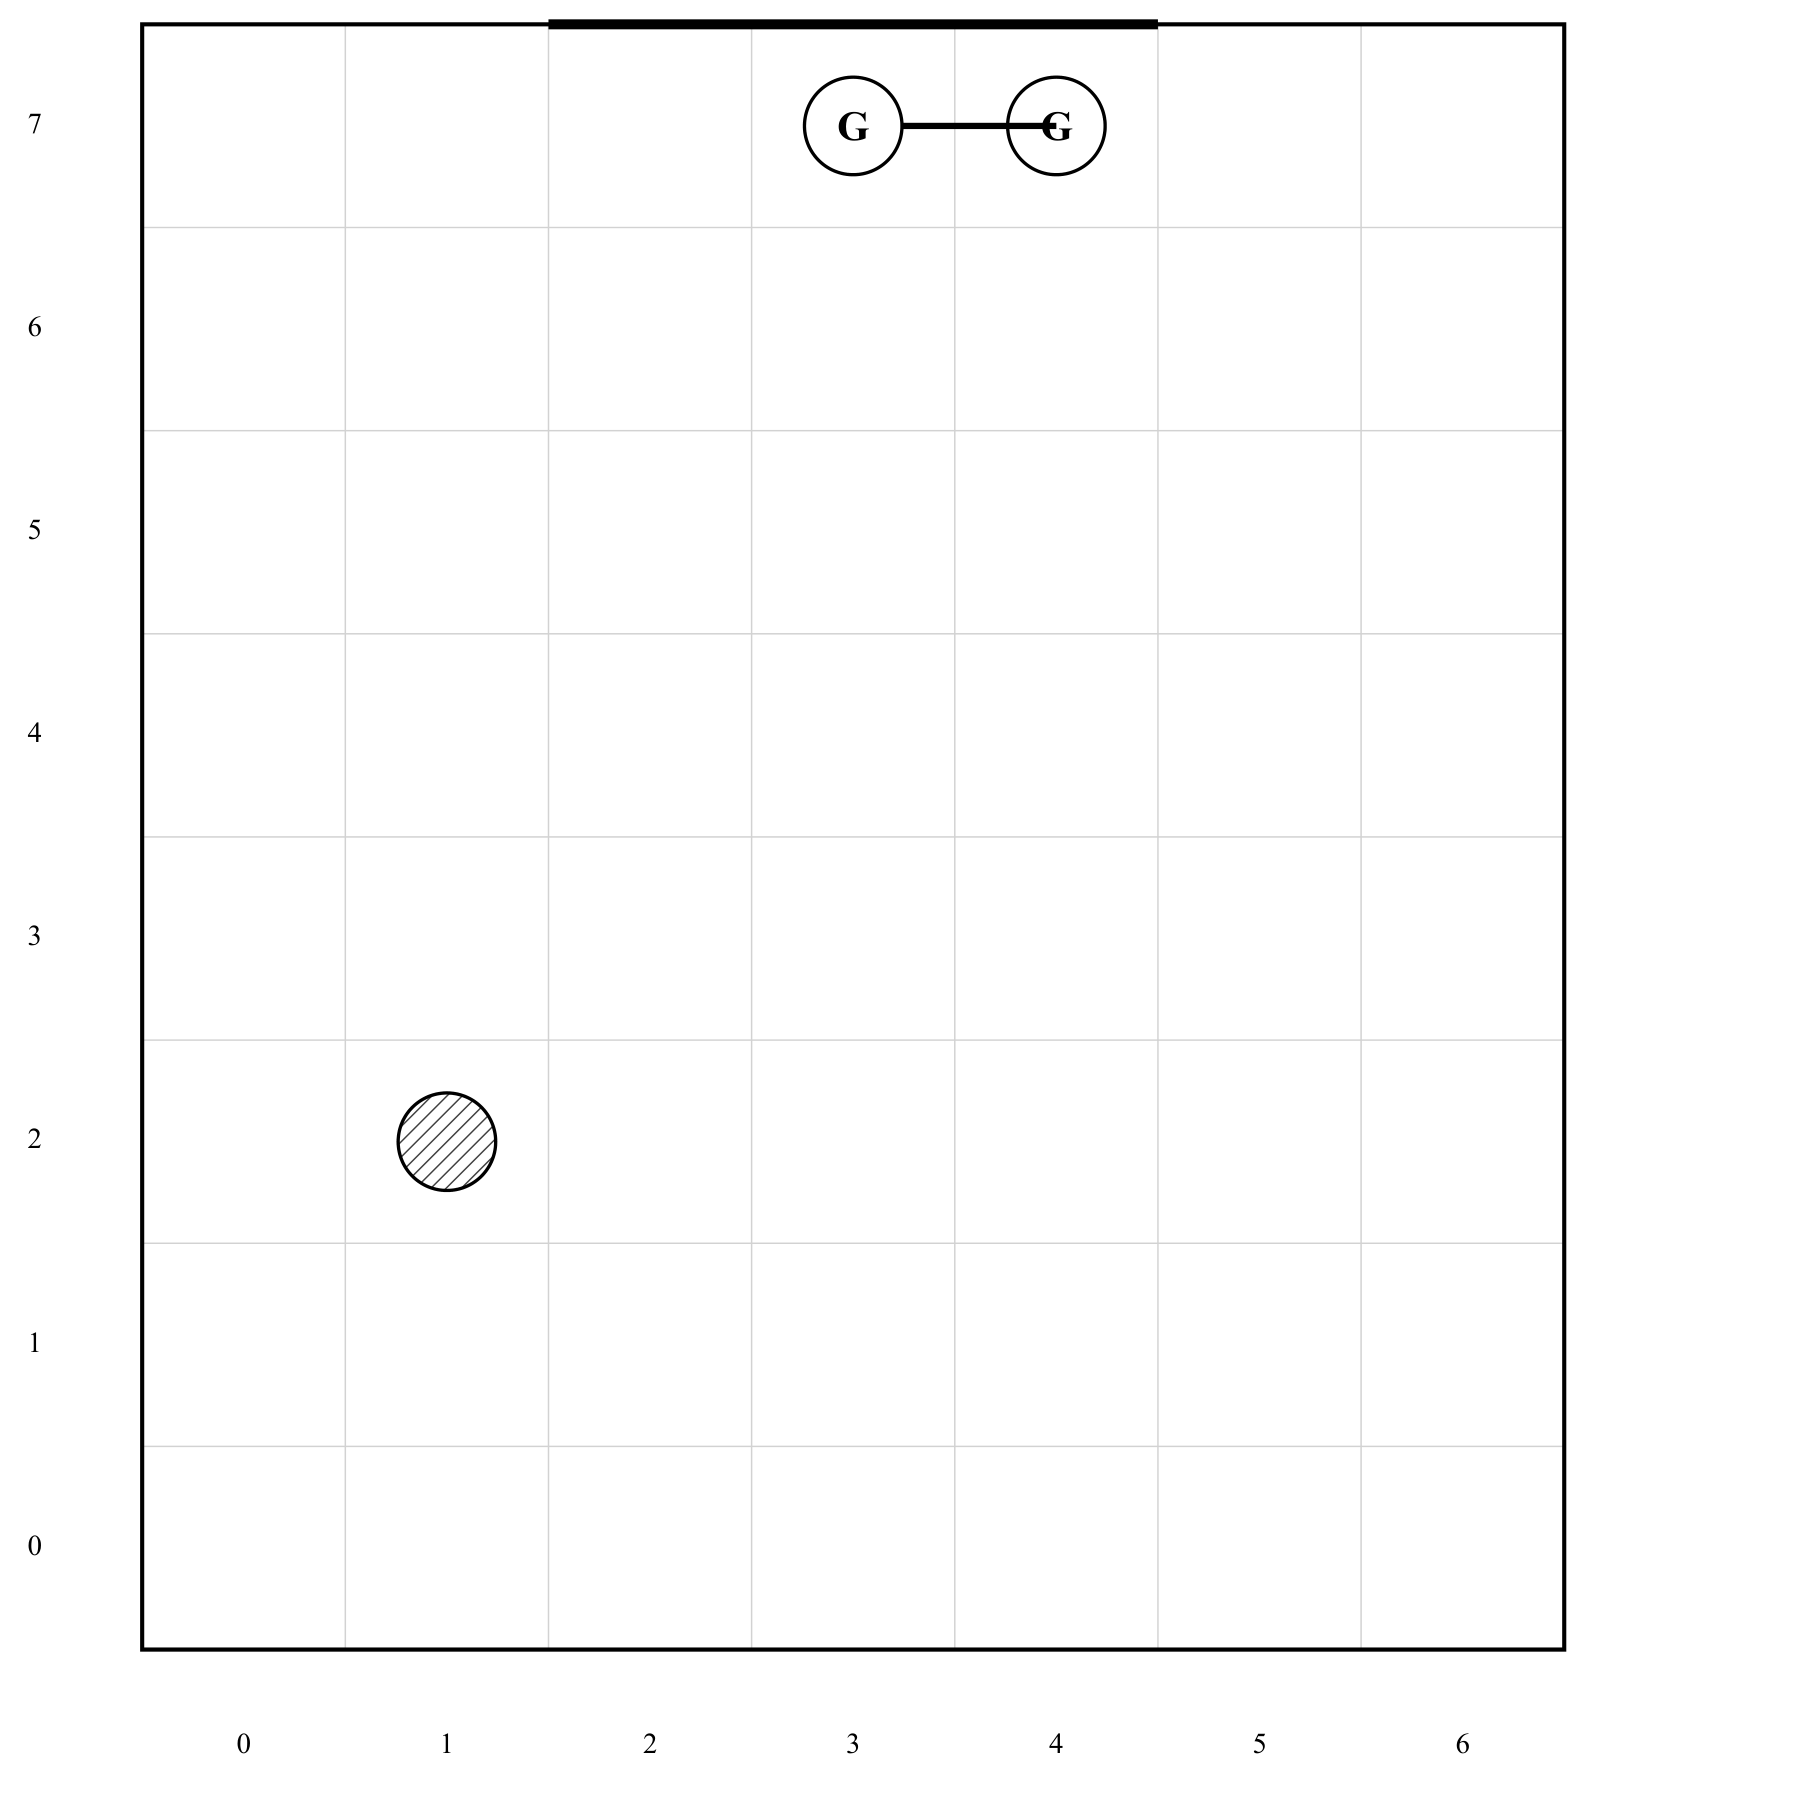
\includegraphics[width=0.82\textwidth]{defender_figures/goalkeeper.png}
\end{center}

\end{document}
